
%(BEGIN_QUESTION)
% Copyright 2014, Tony R. Kuphaldt, released under the Creative Commons Attribution License (v 1.0)
% This means you may do almost anything with this work of mine, so long as you give me proper credit

Read and outline the ``Instrumentation Amplifiers'' subsection and introduction to the ``Analog Signal Conditioning and Referencing'' section of the ``Digital Data Acquisition and Networks'' chapter in your {\it Lessons In Industrial Instrumentation} textbook.  Note the page numbers where important illustrations, photographs, equations, tables, and other relevant details are found.  Prepare to thoughtfully discuss with your instructor and classmates the concepts and examples explored in this reading.

\underbar{file i00882}
%(END_QUESTION)





%(BEGIN_ANSWER)


%(END_ANSWER)





%(BEGIN_NOTES)

Problem to solve: how to match input range of ADC to a given real-world voltage signal?  If the signal is too large, we may use a resistor voltage divider to reduce the signal voltage down to the ADC's range.  If the signal is too small, it will not effectively use the count range of the ADC.  We need to ``condition'' the real-world signal to meet the ADC's input requirements.

\vskip 10pt

Another problem to solve: incompatible grounds.  Sometimes we cannot tie one pole of a real-world voltage signal to ground without causing severe problems, like short-circuits!  Letting the ADC ``float'' at an elevated potential just causes problems on the digital bus side, where the common-mode voltage will interfere with proper interpretation of bit states.  Using a differential amplifier able to handle the common-mode voltage at its inputs solves this problem by ``shifting'' the signal's common mode voltage to zero, translating a ``floating'' differential voltage signal into a ground-referenced voltage signal that the ADC can handle.  A differential amplifier can even boost a weak signal if needed for the ADC's benefit.  Once again, this is a form of ``conditioning'' applied to the signal prior to digitization.

\vskip 10pt

An ``instrumentation amplifier'' is a special differential amplifier equipped with buffered inputs for high input impedance and a gain controllable by a single external resistor.  The gain is typically adjustable between 1 and infinity.  Data Acquisition (DAQ) modules typically have one instrumentation amplifier at each input channel.








\vskip 20pt \vbox{\hrule \hbox{\strut \vrule{} {\bf Suggestions for Socratic discussion} \vrule} \hrule}

\begin{itemize}
\item{} Explain what {\it common-mode} voltage is, and why it can be a problem in data acquisition scenarios.
\item{} Identify a solution for sensing both solar panel voltage and load current that does {\it not} require an instrumentation amplifier.  Hint: relocate the shunt resistor!
\item{} How high should the power supply rail voltages be for the differential amplifier circuit shown in the reading, in order to handle the 33 volt output voltage of the solar panel?
\item{} How practical would it be to use a larger-resistance shunt rather than a differential amplifier {\it with gain} in order to better use the voltage span of the ADC?
\item{} Explain why gain for an instrumentation amplifier increases as $R_G$ decreases, by an examination of the circuit (not simply looking at the gain formula).  The problem-solving strategy of ``limiting cases'' might be useful here.
\item{} Explain the purpose of the ``MUX'' within a DAQ module.  Why do we need a multiplexer inside a data acquisition unit?
\item{} In the ``final solution'' diagram showing the 4-channel DAQ connected to the solar panel circuit, is the 10:1 voltage divider network still necessary?  Explain why or why not.
\item{} In the ``final solution'' diagram showing the 4-channel DAQ connected to the solar panel circuit, which channel should be set for the greater amount of {\it gain}?  Does this require a large $R_G$ or a small $R_G$?
\end{itemize}








\vfil \eject

Calculate all voltage drops and currents given $V_{panel}$, $I_{load}$, and a value for all resistors ($R$) in this circuit:

$$\includegraphics[width=15.5cm]{i00882x01.eps}$$











\vfil \eject

\noindent
{\bf Prep Quiz:}

Explain what {\it common-mode} voltage is.  Be as specific as you can in your answer, and feel free to cite a realistic application if it helps your explanation.












\vfil \eject

\noindent
{\bf Prep Quiz:}

Describe how to alter the gain of an {\it instrumentation amplifier}.  Be as specific as you can in your answer, and feel free to cite a realistic application if it helps your explanation.



%INDEX% Reading assignment: Lessons In Industrial Instrumentation, Digital Data Acquisition and Networks (instrumentation amplifiers)

%(END_NOTES)


